\documentclass[10pt,a4paper]{article}
\usepackage[margin=2.2cm]{geometry}
\usepackage{graphicx,booktabs,amsmath,hyperref,enumitem,xcolor}
\setlist{nosep,leftmargin=1.4em}
\hypersetup{colorlinks,linkcolor=black,urlcolor=blue!50!black}
\title{\textbf{MP2: Selecting Reliable LLM Reasoning}\\[2pt]\large A two-stage verifier over frozen embeddings and answer-level evidence}
\author{DASE7506 Advanced Machine Learning Methods, Fall 2026 \\ Student ID: \texttt{3036797441}}
\date{October 2026}
\begin{document}
\maketitle

\begin{abstract}
For each GSM8K question we must pick one of four Qwen3-0.6B solutions. Majority voting over parsed final answers reaches 69.2\% on the official (hard) test bank. A logistic-regression verifier on \emph{group-centred} frozen embeddings reaches 82.0\%, and a gradient-boosted ranker that combines that score with answer-form, consensus, surface and arithmetic features reaches \textbf{82.44\% (385/467)} on the test bank. The whole prediction + scoring pipeline takes 1.3\,s on CPU and the inference assets are 1.14\,MiB. Ablations show that almost all of the gain over voting comes from the embeddings, used comparatively within a group. Surface features (length, formatting, hedging) are weak on their own. The text-based arithmetic checker adds nothing measurable. The main remaining failure mode is a wrong answer shared by several candidates.
\end{abstract}

\section{Task, data and evaluation protocol}
Each question has four candidate solutions and a fixed 1024-d embedding per candidate. The scorer checks only the parsed final number, and any correct candidate earns the point. Train/validation/test contain 4755/798/467 questions. The test bank keeps only groups with at least two distinct valid parsed answers, so it is much harder than train or validation: majority voting gets 86.2\% on all of validation but 69.2\% on test.

\paragraph{Development protocol.} So that development matches the test distribution, I defined \textbf{validation-hard}: the 355 validation groups with $\ge 2$ distinct valid parsed answers. This filter uses inputs only, never references. All model fitting uses train references only. All design decisions used validation (all and hard) and, for close calls, 5-fold cross-validation on train. The test bank was scored \emph{once}, after the method was frozen. Baselines were scored on test afterwards only for the comparison table. One validation-hard question is worth 0.28\,pp, and the binomial standard error near 82\% is about 2\,pp, so differences under ${\sim}2$\,pp are treated as noise.

\paragraph{What the data looks like.} On validation-hard, 114 groups have exactly one correct candidate, 112 have two and 129 have three. In 60 of the 355 groups the correct answer has \emph{fewer} votes than the plurality answer, so voting cannot get those right. Every reference answer is an integer. Wrong candidates often end in a fraction (e.g.\ ``283.5 students''), produce no parsable answer (truncated after repeated ``let's try again''), or contain hedging language.

\section{Method}
\subsection{Initial method: majority vote}
Parse every candidate with the official \texttt{parse\_answer}, count the votes for each answer, and return the first candidate holding the plurality answer. This method needs no training.

\subsection{Improved method: two-stage verifier}
\textbf{Stage 1: embedding verifier.} For group $g$ with embeddings $e_{g1..4}$, I \emph{centre within the group}, $\tilde e_{gi}=e_{gi}-\frac14\sum_j e_{gj}$, standardise each dimension using train statistics, and fit an L2 logistic regression ($C=0.003$) to predict candidate correctness. Centring removes the question-specific part of the representation; raw embeddings have cosine similarity ${\approx}0.98$ within a group. What remains is how a candidate \emph{differs from its siblings}. On validation-hard, centring alone raised the LR from 76.1\% to 80.0\% (at $C=0.01$). For stacking, train-set stage-1 scores are produced out-of-fold (5 folds, seed 0) so that stage 2 sees honest scores.

\textbf{Stage 2: group ranker.} Each candidate gets 27 hand-crafted features (all computed from inputs only) plus 5 comparative stage-1 features:
\begin{itemize}
\item \emph{Answer form} (8): no parse, integer, negative, zero, $\log$ magnitude, answer copied from the question, share of question numbers reused, last number in the text equals the parsed answer.
\item \emph{Consensus} (6): vote share, is/uniquely is the plurality, number of distinct answers, number of unparsable siblings, vote rank.
\item \emph{Surface} (9): characters, lines, number of \verb|\boxed|, \texttt{\#\#\#\#} present, ``Step'' headers, hedge-word count (``wait'', ``try again'', ``mistake'', ``assume'', \dots), count of numbers, share of numbers taken from the question, length relative to the group.
\item \emph{Arithmetic} (4): a small LaTeX-aware checker evaluates each ``\textit{expr} = \textit{expr}'' step (handling \verb|\times|, \verb|\frac|, \verb|\div|, thousands separators, \verb|\text{}|). It records checked steps, wrong steps, any-wrong and wrong fraction.
\item \emph{Comparative stage-1} (5): logit, logit minus the group max, logit minus the group mean, summed probability of candidates sharing the same answer (``soft voting''), and margin to the best candidate with a \emph{different} answer.
\end{itemize}
A \texttt{HistGradientBoostingClassifier} (300 iterations, learning rate 0.05, 15 leaves, L2 = 1) predicts correctness. Three seeds are averaged, and the highest-scoring candidate is chosen, with ties going to the lowest index. Training takes 5\,s on a laptop CPU, and retraining reproduces the checkpoint bit-for-bit.

\subsection{Variants that were tried and rejected}
\begin{itemize}
\item \emph{Pairwise (RankNet-style) linear model on embedding differences}: 80.3\% val-hard, no better than pointwise.
\item \emph{Listwise softmax over the four candidates}: 76.1\%.
\item \emph{MLP on embeddings}: 73.5\% alone; it overfits.
\item \emph{TF-IDF word uni/bi-gram LR over the full text} (hashed, $2^{16}$ dims): only 58.9\% val-hard, worse than voting, and $+0.3$\,pp when stacked.
\item \emph{Answer-level pooling of stage-2 features}: 82.8--84.2\% across seeds, the same as the candidate level.
\item \emph{Training only on hard groups}: no gain.
\end{itemize}
I kept the simplest variant that was at least as good.

\paragraph{Second optimisation round (after freezing; judged on train-CV and validation only).}
I ran a second round of experiments after the method was frozen. Each candidate change was judged by 5-fold CV on the 2114 hard train groups (standard error ${\approx}0.85$\,pp) and by validation-hard. No change to the frozen model was adopted, so the test bank was not re-scored.
\begin{itemize}
\item \emph{Cross-candidate text evidence} (my answer appears in a rival's reasoning, rival answers appear in mine, how often I restate my answer): CV $-0.1$, val-hard $+1.1$.
\item \emph{Answer-cluster logit statistics}: CV $+0.3$, val-hard $-0.6$.
\item \emph{A second stage-1 model on raw embeddings}: CV $-0.2$, val-hard $-0.6$.
\item \emph{Four ranker hyper-parameter settings}: CV within $\pm0.15$.
\item \emph{Alternative stage-1 models} (shrinkage LDA, $\ell_2$-normalised inputs, PCA with squared terms, a 3-model ensemble), compared on stage-1 accuracy alone: CV-hard ranged from 74.3\% to 79.8\%, against 79.2\% for the frozen centred LR.
\end{itemize}
Every change stayed within one standard error, or its CV and validation results moved in opposite directions. Adopting the validation winner (cross features) would have meant fitting to noise in 355 questions. The evidence suggests that a \emph{linear read-out of the frozen embeddings is saturated} at about 80\% on hard groups. Further gains would need information that is not in the inputs, such as re-solving the problem, which the offline rule forbids. Logs: \texttt{code/results/opt\_round2.txt} and \texttt{opt\_emb\_round2.txt}.

\paragraph{Third round, targeting the observed failure modes.} The error analysis suggested two more ideas.
\begin{itemize}
\item \emph{Missed conditions.} I measured how many of the question's quantities a solution actually uses, counting digits, number words such as ``twice'' or ``dozen'', and percentages. I also measured how far an answer's magnitude is from the group median. Both features do separate the classes: wrong candidates leave 0.25 conditions unused against 0.18 for correct ones, and their magnitude deviation is 0.31 against 0.10.
\item \emph{Retrieval.} I scored each candidate by the correctness of its 50 nearest train candidates in a 64-d PCA space.
\end{itemize}
Neither moved the selection result, averaged over two CV seeds. Coverage gave 81.79\% against a baseline of 81.79\%, and kNN gave 81.65\%. kNN alone reached only 67.9\% on val-hard. The coverage signal is apparently already captured by the embedding margin and the existing answer features. Retrieval fails because nearby train questions do not share the current question's failure mode. The model was therefore not changed (log: \texttt{code/results/opt\_round3.txt}).

\section{Results}
\begin{table}[h]\centering\small
\begin{tabular}{lcccc}\toprule
Method & Val (all, 798) & Val-hard (355) & \textbf{Test (467)} & Assets \\ \midrule
First candidate & 78.20 & 54.93 & -- & 0 \\
Majority vote (initial) & 86.22 & 69.01 & 69.16 & 0 \\
Embedding LR only (stage 1) & 91.10 & 81.41 & 82.01 & 13 KB \\
Hand features only (stage 2, no embeddings) & 90.23 & 78.03 & -- & -- \\
\textbf{Full two-stage verifier (frozen)} & \textbf{92.86} & \textbf{83.94} & \textbf{82.44} & 1.14 MiB \\
Oracle (any correct candidate) & 100 & 100 & 100 & -- \\ \bottomrule
\end{tabular}
\caption{Selection accuracy (\%). Test numbers come from the official scorer, after freezing. Baseline test runs use \texttt{baselines/*.py} through the official \texttt{predict.py}.}
\end{table}

\noindent On test, the frozen method gains $+13.3$\,pp over majority voting (62 more questions). Compared with stage 1 alone it gains only $+0.43$\,pp (2 questions). On validation-hard the stage-2 gain was $+2.5$\,pp. Section~\ref{sec:cost} discusses whether stage 2 is worth its cost. 5-fold CV on train agrees: emb-only scores 79.2\% on the 2114 hard train groups and the full model 81.7\%.

\begin{figure}[h]\centering
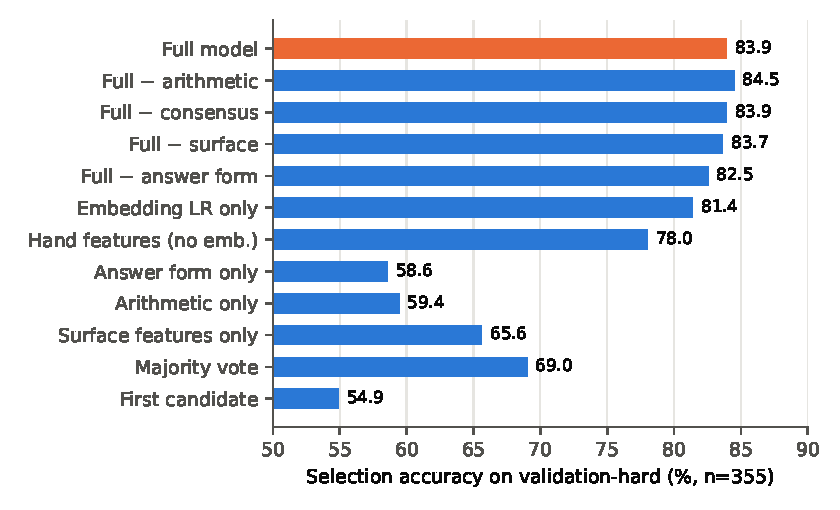
\includegraphics[width=0.66\linewidth]{figures/ablation.pdf}
\caption{Feature-group ablations on validation-hard. ``$X$ only'' uses a ranker on that group alone, without embeddings. ``Full $-X$'' removes group $X$ from the frozen model.}
\label{fig:abl}
\end{figure}

\section{Analysis}
\subsection{Does reading the reasoning help, or just length and formatting?}
Figure~\ref{fig:abl} separates the explanations. A ranker on \emph{surface features alone} (length, line count, boxing, step headers, hedges) reaches 65.6\% on val-hard, below voting. Removing surface features from the full model costs only 0.3\,pp. Length barely differs between correct and wrong candidates on val-hard (mean $\log$ chars 6.24 vs 6.22). So the method does not mainly rely on length or formatting. The one ``style'' signal that matters is \emph{hedging}: wrong candidates contain 4$\times$ more hedge words (0.22 vs 0.05 per solution), because the 0.6B model often flounders before it guesses. Bag-of-words over the full reasoning is \emph{worse} than voting (58.9\%), so shallow text reading does not recover reasoning quality.

The \textbf{embeddings carry most of the signal}. On permutation importance, the single most important input is the stage-1 \emph{margin to the best different-answer candidate}: shuffling it costs 8.6\,pp. The next is \texttt{ans\_int} (2.3\,pp), a task prior that every GSM8K answer is an integer. The arithmetic checker disagrees with the hypothesis that wrong answers come from wrong arithmetic. Only 15.1\% of wrong candidates on val-hard contain a detected wrong step, against 10.3\% of correct ones, and removing the group changes accuracy by $+0.6$\,pp (noise; train-CV $+0.1$\,pp). This matches the guide's example: most errors are \emph{setup} errors (a wrong interpretation, a missed condition) with correct arithmetic, and a step checker cannot see those.

\subsection{Should a candidate be judged alone?}
No. Group-centring raises the embedding LR from 76.1\% to 80.0\%, and every useful stage-1 input to the ranker is comparative (margin, relative-to-max, answer-sum). Pure consensus is also comparative. It is strong on easy groups but caps out on hard ones: voting cannot solve the 60 val-hard groups where the right answer is a minority. The full model solves 46.7\% of those. Consensus features add nothing once the soft vote (\texttt{emb\_answer\_sum}) is present: removing them changes accuracy by 0.0\,pp.

\subsection{Does the method know when it is uncertain?}
\begin{figure}[h]\centering
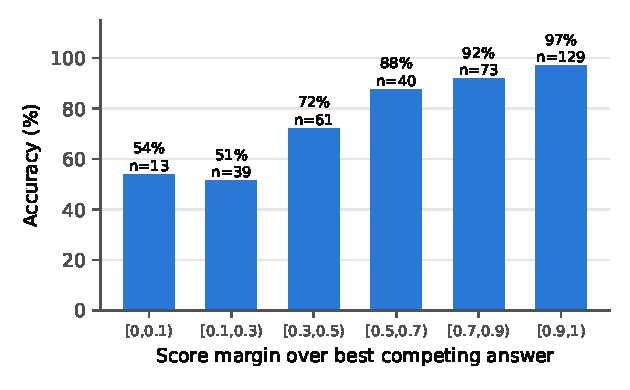
\includegraphics[width=0.5\linewidth]{figures/calibration.pdf}
\caption{Validation-hard accuracy against the score margin between the chosen answer and the best competing answer.}
\label{fig:cal}
\end{figure}
Yes, fairly well (Fig.~\ref{fig:cal}). When the margin over the best competing answer is below 0.3, accuracy is about 52\% (52 questions). Above 0.9 it is 96.9\% (129 questions). If the method answered only its most confident 50\% of val-hard questions it would reach 95.5\%, and its most confident 25\% would reach 100\%. Disagreement between methods is also informative. When the full model, voting and stage 1 all agree (67.6\% of val-hard), accuracy is 90.8\%. Otherwise it is 69.6\%. When the full model overrides the majority (90 questions) it is right 72.2\% of the time, while voting gets only 13.3\% of those 90 right.

\subsection{Where does it fail?}
Accuracy on val-hard is 56.1\% when exactly one candidate is correct, 93.8\% with two and 100\% with three. Of the 57 validation errors, 49 chose a plurality answer, i.e.\ several samples converged on the same wrong interpretation. Typical examples: ``produces 2 baby plants 2 times a year, after 4 years'', where two candidates answer 4, one 8 and the correct one 16; or an averaging question where four candidates give four different answers. When the evidence is one lone candidate against agreeing siblings, the frozen embeddings, which come from a 0.6B model with the same blind spots, rarely override the crowd. Going further would need re-solving or executing the problem, which the offline rule forbids.

\subsection{When does more computation pay off?}\label{sec:cost}
\begin{table}[h]\centering\small
\begin{tabular}{lccc}\toprule
Method & Test acc. & Inference assets & Train cost \\ \midrule
Majority vote & 69.16 & 0 & none \\
Embedding LR & 82.01 & 13\,KB & $<$1\,s \\
Full verifier, 1 ranker seed & (val-hard 83.94) & 0.32\,MiB & ${\sim}$2\,s \\
Full verifier, 3 ranker seeds (frozen) & 82.44 & 1.14\,MiB & 5\,s \\ \bottomrule
\end{tabular}
\end{table}
The large jump (+12.9\,pp) costs 8\,KB of weights and a matrix product. Stage 2 adds feature extraction (${\approx}0.5$\,s for 467 questions) and 1.1\,MiB. It gave +2.5\,pp on val-hard and +2.5\,pp in train-CV, but only +0.4\,pp on test, which is within noise. The three-seed ensemble gave 0.0\,pp on validation and +0.4\,pp in CV, so it mostly repeats the same mistakes at higher cost. I kept the three seeds because that choice was fixed before testing and the cost is negligible. An honest summary: the extra machinery pays off modestly, and the embeddings with a comparative read-out do most of the work.

\section{Resources and reproducibility}
\begin{itemize}
\item \textbf{Hardware (local):} Apple M5 (10 cores), macOS. Python 3.12.15, numpy 2.5.3, scikit-learn 1.9.1, scipy 1.18.1, joblib 1.6.0, threadpoolctl 3.7.0 (\texttt{code/requirements.txt}).
\item \textbf{Timing:} one fresh \texttt{predict.py} plus \texttt{score\_predictions.py} on the full test bank with \texttt{OMP/OPENBLAS/MKL\_NUM\_THREADS=4}, measured externally with \texttt{/usr/bin/time}: \textbf{1.34\,s wall}. The runner reports 1.09\,s for prediction and 0.011\,s for scoring. This is far below the 30\,s limit, and an x86 Xeon should be in the same range.
\item \textbf{Assets:} \texttt{checkpoint/model\_bundle/}: \texttt{verifier.npz} 13{,}286\,B, \texttt{rankers.pkl} 1{,}183{,}688\,B, \texttt{config.json} 787\,B. Total 1.14\,MiB, under 16\,MiB. SHA-256 hashes are in \texttt{SUBMISSION.md}.
\item \textbf{Seeds:} KFold seed 0, ranker seeds 0/1/2. Retraining reproduces identical file hashes and identical test predictions.
\item \textbf{Data use:} training references only for fitting; validation for selection; test references only for the final official score.
\end{itemize}

\section{AI and reuse disclosure}
AI coding assistance (Claude, Anthropic) was used substantively: to write the feature extractor, the training and analysis scripts and a draft of this report. I reviewed the code and results. No external datasets, pretrained weights, generated text or third-party code beyond numpy/scikit-learn/matplotlib were used.

\end{document}
